\documentclass[tikz,border=10pt]{standalone}
\usepackage[utf8]{inputenc}
\usepackage{tikz}
\usepackage{colortbl}
\usetikzlibrary{shapes,arrows.meta,positioning,calc,fit}

\definecolor{ScoutGreen}{HTML}{005432}
\definecolor{ScoutNavy}{HTML}{002855}
\definecolor{ScoutBlue}{HTML}{006EB6}
\definecolor{ScoutRed}{HTML}{A31920}
\definecolor{ScoutAmber}{HTML}{D97706}
\definecolor{BorderGray}{HTML}{CBD5E1}

\begin{document}
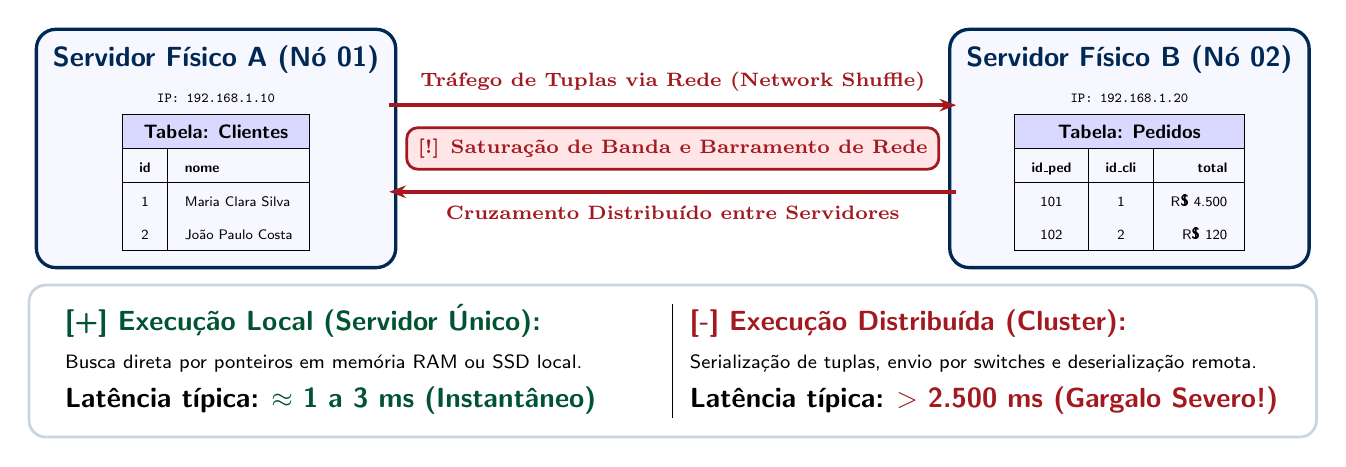
\begin{tikzpicture}[
    font=\sffamily,
    srvbox/.style={draw=ScoutNavy, rounded corners=7pt, fill=blue!3, line width=1.2pt, inner sep=6pt, align=center},
    arrow/.style={-{Stealth[length=6pt]}, line width=1.5pt}
]

  % -------------------------------------------------------------
  % SERVIDOR 01 (NÓ A) - y = 1.5, x = 0
  % -------------------------------------------------------------
  \node[srvbox, minimum width=4.2cm] (srv1) at (0, 1.5) {
    \textbf{\textcolor{ScoutNavy}{Servidor Físico A (Nó 01)}}\\[1pt]
    \tiny \texttt{IP: 192.168.1.10}\\[3pt]
    \begin{tabular}{|c|l|}
      \hline
      \multicolumn{2}{|c|}{\cellcolor{blue!15}\scriptsize\textbf{Tabela: Clientes}} \\
      \hline
      \tiny\textbf{id} & \tiny\textbf{nome} \\
      \hline
      \tiny 1 & \tiny Maria Clara Silva \\
      \tiny 2 & \tiny João Paulo Costa \\
      \hline
    \end{tabular}
  };

  % -------------------------------------------------------------
  % SERVIDOR 02 (NÓ B) - y = 1.5, x = 11.6
  % -------------------------------------------------------------
  \node[srvbox, minimum width=4.2cm] (srv2) at (11.6, 1.5) {
    \textbf{\textcolor{ScoutNavy}{Servidor Físico B (Nó 02)}}\\[1pt]
    \tiny \texttt{IP: 192.168.1.20}\\[3pt]
    \begin{tabular}{|c|c|r|}
      \hline
      \multicolumn{3}{|c|}{\cellcolor{blue!15}\scriptsize\textbf{Tabela: Pedidos}} \\
      \hline
      \tiny\textbf{id\_ped} & \tiny\textbf{id\_cli} & \tiny\textbf{total} \\
      \hline
      \tiny 101 & \tiny 1 & \tiny R\$ 4.500 \\
      \tiny 102 & \tiny 2 & \tiny R\$ 120 \\
      \hline
    \end{tabular}
  };

  % -------------------------------------------------------------
  % CANAL DE REDE E NETWORK SHUFFLE (ESPAÇO CENTRAL 7.4cm)
  % -------------------------------------------------------------
  % Seta superior (A -> B)
  \draw[arrow, color=ScoutRed] (2.2, 2.05) -- (9.4, 2.05)
    node[midway, above, font=\scriptsize\bfseries, text=ScoutRed, yshift=1pt] {Tráfego de Tuplas via Rede (Network Shuffle)};

  % Box central de alerta
  \node[draw=ScoutRed, fill=red!10, rounded corners=4pt, line width=1pt, inner sep=4pt, font=\scriptsize\bfseries, text=ScoutRed] at (5.8, 1.5) {
    [!] Saturação de Banda e Barramento de Rede
  };

  % Seta inferior (B -> A)
  \draw[arrow, color=ScoutRed] (9.4, 0.95) -- (2.2, 0.95)
    node[midway, below, font=\scriptsize\bfseries, text=ScoutRed, yshift=-1pt] {Cruzamento Distribuído entre Servidores};

  % -------------------------------------------------------------
  % CARD COMPARATIVO INFERIOR (y = -1.2, TOTALMENTE SEPARADO)
  % -------------------------------------------------------------
  \node[draw=BorderGray, fill=white, rounded corners=6pt, line width=1pt, minimum width=15.8cm, inner sep=7pt] at (5.8, -1.2) {
    \begin{tabular}{p{7.5cm} | p{7.5cm}}
      \textbf{\textcolor{ScoutGreen}{[+] Execução Local (Servidor Único):}} & \textbf{\textcolor{ScoutRed}{[-] Execução Distribuída (Cluster):}} \\[2pt]
      \scriptsize Busca direta por ponteiros em memória RAM ou SSD local. & \scriptsize Serialização de tuplas, envio por switches e deserialização remota. \\[2pt]
      \textbf{Latência típica:} \textcolor{ScoutGreen}{\textbf{$\approx$ 1 a 3 ms (Instantâneo)}} & \textbf{Latência típica:} \textcolor{ScoutRed}{\textbf{$>$ 2.500 ms (Gargalo Severo!)}} \\
    \end{tabular}
  };

\end{tikzpicture}
\end{document}
